\documentclass[border=15pt, multi, tikz]{standalone}
%\usepackage{blocks}
\usepackage{import}
\subimport{../../layers/}{init}
\usetikzlibrary{positioning}
\usetikzlibrary{3d}

\def\ConvColor{rgb:yellow,5;red,2.5;white,5}
\def\ConvReluColor{rgb:yellow,5;red,5;white,5}
\def\PoolColor{rgb:red,1;black,0.3}
\def\FcColor{rgb:blue,5;red,2.5;white,5}
\def\FcReluColor{rgb:blue,5;red,5;white,4}
\def\SoftmaxColor{rgb:magenta,5;black,7}

\begin{document}
\begin{tikzpicture}
\tikzstyle{connection}=[ultra thick,every node/.style={sloped,allow upside down},draw=\edgecolor,opacity=0.7]
%%%%%%%%%%%%%%%%%%%%%%%%%%%%%%%%%%%%%%%%%%%%%%%%%%%%%%%%%%%%%%%%%%%%%%%%%%%%%%%%%%%%%%%%
%% Draw Layer Blocks
%%%%%%%%%%%%%%%%%%%%%%%%%%%%%%%%%%%%%%%%%%%%%%%%%%%%%%%%%%%%%%%%%%%%%%%%%%%%%%%%%%%%%%%%
\node[canvas is zy plane at x=0] (temp) at (-2,0,0) {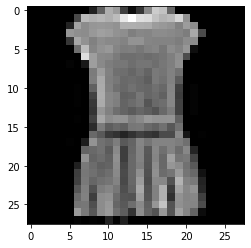
\includegraphics[width=8cm,height=8cm]{dress.png}};

% conv1_1,conv1_2
\pic[shift={(0,0,0)}] at (0,0,0) {RightBandedBox={name=cr1,%
        xlabel={{"1",""}},ylabel=28,zlabel=28,fill=\ConvColor,bandfill=\ConvReluColor,%
        height=40,width={2},depth=40}};
%kernel 
\pic[shift={(0,0,0)}] at (0,0,0) {RightBandedBox={name=k,caption=k,%
        xlabel=1,ylabel=3, zlabel= 3,fill=\ConvColor,bandfill=\ConvReluColor,%
        height=10,width=1,depth=10}};
%conv_out
\pic[shift={(1.5,0,0)}] at (k-east){Box={name=out1,caption=conv1,xlabel={{"","","","12","","",""}},%
        fill=\SoftmaxColor,opacity=0.5,height=40,width={1,1,1,1,1,1,1},depth=40}};
%Maxpool1        
\pic[shift={(1.5,0,0)}] at (out1-east) {Box={name=p1, caption = maxpool, xlabel={{"","","","12","","",""}},%
        fill=\PoolColor,opacity=0.5,height=14,width={1,1,1,1,1,1,1},depth=14}};
%kernel
\pic[shift={(0,0,0)}] at (p1-east) {RightBandedBox={name=k,caption=k,%
        xlabel=1,ylabel=3, zlabel= 3,fill=\ConvColor,bandfill=\ConvReluColor,%
        height=10,width=1,depth=10}};
% conv5_1,conv5_2,conv5_3
\pic[shift={(2,0,0)}] at (p1-east) {RightBandedBox={name=cr5,caption=conv2,%
        xlabel={{"","","","","","","24","","","","","","",""}}, ylabel = 12,zlabel=12,fill=\ConvColor,bandfill=\ConvReluColor,%
        height=12,width={1,1,1,1,1,1,1,1,1,1,1,1,1,1},depth=12}};
%pool5
\pic[shift={(1.5,0,0)}] at (cr5-east) {Box={name=p5, caption=maxpool,%
        fill=\PoolColor,opacity=0.5, xlabel={{"","","","","","","24","","","","","","",""}}, zlabel = 6, ylabel = 6,height=6,width={1,1,1,1,1,1,1,1,1,1,1,1,1,1},depth=6}};
%%%%%%%%%%
% fc6
\pic[shift={(2,0,0)}] at (p5-east) {RightBandedBox={name=fc6,caption=fc1,%
        xlabel={{"1",""}},zlabel=600,fill=\FcColor,bandfill=\FcReluColor,%
        height=3,width=2,depth=40}};
%%%%%%%%%%
% fc7
\pic[shift={(2,0,0)}] at (fc6-east) {RightBandedBox={name=fc7,caption=fc2,%
        xlabel={{"1","dummy"}},zlabel=100,fill=\FcColor,bandfill=\FcReluColor,%
        height=3,width=2,depth=30}};
%%%%%%%%%%
% fc8
\pic[shift={(1.5,0,0)}] at (fc7-east) {RightBandedBox={name=fc8,caption=fc3,%
        xlabel={{"1","dummy"}}, zlabel = 10,fill=\FcColor,bandfill=\FcReluColor,%
        height=3,width=2,depth=10}};

    
%%%%%%%%%%%%%%%%%%%%%%%%%%%%%%%%%%%%%%%%%%%%%%%%%%%%%%%%%%%%%%%%%%%%%%%%%%%%%%%%%%%%%%%%
%% Draw Arrow Connections
%%%%%%%%%%%%%%%%%%%%%%%%%%%%%%%%%%%%%%%%%%%%%%%%%%%%%%%%%%%%%%%%%%%%%%%%%%%%%%%%%%%%%%%%
\draw [connection]  (cr1-east)       -- node {\midarrow} (p1-east);
\draw [connection]  (p1-east)        -- node {\midarrow} (cr5-east);
\draw [connection]  (cr5-east)       -- node {\midarrow} (p5-west);
\draw [connection]  (p5-east)        -- node {\midarrow} (fc6-east);
\draw [connection]  (fc6-east)       -- node {\midarrow} (fc7-west);
\draw [connection]  (fc7-east)       -- node {\midarrow} (fc8-west);
%%%%%%%%%%%%%%%%%%%%%%%%%%%%%%%%%%%%%%%%%%%%%%%%%%%%%%%%%%%%%%%%%%%%%%%%%%%%%%%%%%%%%%%%
%% Draw Dotted Edges 
%%%%%%%%%%%%%%%%%%%%%%%%%%%%%%%%%%%%%%%%%%%%%%%%%%%%%%%%%%%%%%%%%%%%%%%%%%%%%%%%%%%%%%%%
\draw[densely dashed]
    (fc6-west)++(0, 1.5*.2, 1.5*.2) coordinate(a) -- (p5-nearnortheast)
    (fc6-west)++(0,-1.5*.2, 1.5*.2) coordinate(b) -- (p5-nearsoutheast)
    (fc6-west)++(0,-1.5*.2,-1.5*.2) coordinate(c) -- (p5-farsoutheast)
    (fc6-west)++(0, 1.5*.2,-1.5*.2) coordinate(d) -- (p5-farnortheast)
    
    (a)--(b)--(c)--(d)
    ;
    %;
%%%%%%%%%%%%%%%%%%%%%%%%%%%%%%%%%%%%%%%%%%%%%%%%%%%%%%%%%%%%%%%%%%%%%%%%%%%%%%%%%%%%%%%%
\end{tikzpicture}
\end{document}